\documentclass[12pt]{article}
\usepackage[margin=1in]{geometry}
\usepackage{graphicx}
\usepackage{caption}
\usepackage{float}
\usepackage{setspace}
\usepackage{booktabs}
\usepackage{siunitx}
\usepackage{amsmath, amssymb}
\usepackage{hyperref}
\hypersetup{colorlinks=true,linkcolor=blue,urlcolor=blue,citecolor=blue}
\sisetup{per-mode=symbol,detect-all=true}
\onehalfspacing
\title{A Computational Analysis of a Set Parameter Beta-Type Stirling Engine\\and Flywheel Design Optimization}
\author{Thomas Ritten \and Sebastian Hondl \and Peyton Lettau}
\date{Group 29 -- ME4051 -- 9/20/25}
\begin{document}
\maketitle
\section*{Abstract}
The effectiveness of an energy conversion system is often defined by its losses: what causes them, how significant they are, and how they can be reduced to improve overall system performance. For Beta-type Stirling engines, we examine work generation in real versus ideal conditions, torque balance across the cycle, crankshaft speed fluctuation, and phase angle sensitivity. We also size a flywheel to meet a target coefficient of fluctuation given material and geometric constraints.

\section{Introduction}
Stirling engines provide a straightforward yet effective method of converting heat into mechanical work. To evaluate performance, we analyze each phase of the cycle versus crank angle \(\theta\), comparing pressure, volume, work, and torque distributions. Beyond the thermodynamic cycle, the flywheel must supply sufficient inertia to maintain near-constant angular velocity without overloading the system.

\section{Given Parameters}
Key parameters used throughout the analysis are summarized below.
\begin{table}[H]
  \centering
  \caption{Initial engine and operating parameters (given).}
  \label{tab:params}
  \begin{tabular}{@{}llll@{}}
    \toprule
    \textbf{Parameter} & \textbf{Symbol} & \textbf{Value} & \textbf{Units} \\
    \midrule
    Power piston crank length & $r_{p}$ & \num{0.025} & \si{\meter} \\
    Power piston connecting rod & $\ell_{p}$ & \num{0.075} & \si{\meter} \\
    Displacer crank length & $r_{d}$ & \num{0.02} & \si{\meter} \\
    Displacer connecting rod & $\ell_{d}$ & \num{0.14} & \si{\meter} \\
    Displacer volume & $V_{d}$ & \num{4.0e-5} & \si{\meter\cubed} \\
    Cylinder bore diameter & $D$ & \num{0.05} & \si{\meter} \\
    Phase shift & $\phi$ & $\pi/2$ & \si{\radian} \\
    Compression ratio & $\mathrm{CR}$ & \num{1.7} & --- \\
    Hot temperature & $T_{h}$ & \num{900} & \si{\kelvin} \\
    Cold temperature & $T_{c}$ & \num{300} & \si{\kelvin} \\
    Gas pressure at BDC & $P_{\mathrm{BDC}}$ & \num{500} & \si{\kilo\pascal} (abs) \\
    Atmospheric pressure & $P_{\mathrm{atm}}$ & \num{101.3} & \si{\kilo\pascal} (abs) \\
    Regenerator dead volume & $V_{\mathrm{reg}}$ & \num{2.0e-5} & \si{\meter\cubed} \\
    Flywheel width & $w$ & \num{0.025} & \si{\meter} \\
    Flywheel rim thickness & $t$ & \num{0.05} & \si{\meter} \\
    Flywheel material density & $\rho$ & \num{8000} & \si{\kilo\gram\per\meter\cubed} \\
    Coefficient of fluctuation & $C_{f}$ & \num{0.003} & --- \\
    Average rotational speed & $\overline{\Omega}$ & \num{650} & \si{rpm} \\
    \bottomrule
  \end{tabular}
\end{table}

\section{Stirling Engine Overview}
Figure~\ref{fig:stirling} shows the Beta-type Stirling engine schematic used in this study.
\begin{figure}[H]
  \centering
  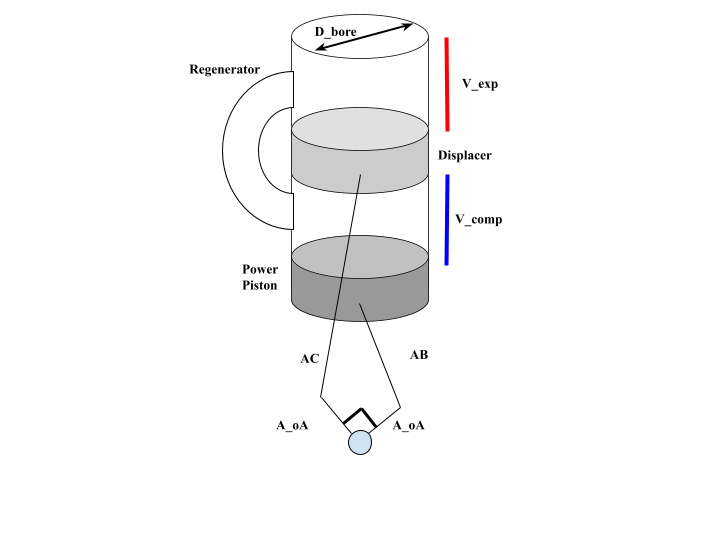
\includegraphics[width=0.9\linewidth]{figures/stirling.png}
  \caption{Stirling engine diagram.}
  \label{fig:stirling}
\end{figure}
\section{Methodology}
We discretize the crank angle as \(\theta \in [0,2\pi)\) with 360 evenly spaced points. With equal bore diameters, the cross-sectional area is \(A = \pi D^{2}/4\).

\subsection{Slider--Crank Kinematics}
Piston/displacer positions follow the slider--crank with rod obliquity. For a crank radius \(r\) and rod length \(\ell\):
\begin{align}
  \beta(\theta) &= \arcsin\!\biggl( \frac{r}{\ell}\,\sin\theta \biggr),\label{eq:beta-def}\\
  x(\theta) &= \ell\,\cos\beta(\theta) - r\,\cos\theta.
\end{align}
We use \(x_{p}(\theta)\) for the power piston and \(x_{d}(\theta+\phi)\) for the displacer (phase shifted by \(\phi\)).

\subsection{Cold/Hot Volumes}
Cold height is the separation between displacer and power piston minus fixed offsets; hot height is measured from the top space above the displacer:
\begin{align}
  h_{c}(\theta) &= \bigl[x_{d}(\theta+\phi) - x_{p}(\theta)\bigr] - h_{\mathrm{pin}} - \tfrac{1}{2}h_{d},\\
  h_{h}(\theta) &= H_{\mathrm{tot}} - \tfrac{1}{2}h_{d} - x_{d}(\theta+\phi),
\end{align}
with volumes
\begin{align}
  V_{c}(\theta) &= A\,h_{c}(\theta), & V_{h}(\theta) &= A\,h_{h}(\theta), & V_{r} &= \text{const}.
\end{align}

\subsection{Schmidt Analysis and Mass from BDC}
Let \(T_{c},T_{h},T_{r}\) be cold, hot, and regenerator temperatures and \(R\) the specific gas constant. Total mass is fixed and determined at BDC (\(\theta=0\)) using the known absolute pressure \(P_{\mathrm{BDC}}\):
\begin{align}
  m &= \frac{P_{\mathrm{BDC}}}{R}\biggl( \frac{V_{c}(0)}{T_{c}} + \frac{V_{r}}{T_{r}} + \frac{V_{h}(0)}{T_{h}} \biggr).
\end{align}
Instantaneous absolute pressure then follows the Schmidt relation
\begin{align}
  P(\theta) &= \frac{m\,R}{\dfrac{V_{c}(\theta)}{T_{c}} + \dfrac{V_{r}}{T_{r}} + \dfrac{V_{h}(\theta)}{T_{h}} }.
\end{align}
Cycle work is evaluated numerically as
\begin{equation}
  W = \oint P\,\mathrm{d}V \approx \sum_{k} P(\theta_{k})\,\Delta V(\theta_{k}) \quad \text{(trapezoidal rule)}.
\end{equation}

\subsection{Torque with Rod Obliquity}
Net axial force on the power piston is \(F_{p}(\theta) = \bigl(P(\theta)-P_{\mathrm{atm}}\bigr)\,A\). With \(\beta\) from Eq.~\eqref{eq:beta-def} and crank radius \(r_{p}\), the torque is
\begin{equation}
  \tau(\theta) = -\,F_{p}(\theta)\,\frac{r_{p}\,\sin\theta}{\cos\beta(\theta)}.
\end{equation}
The displacer contributes zero torque (equal pressure both sides, zero rod area).

\subsection{Flywheel Sizing}
Let \(\omega_{\!\text{avg}}\) be the average angular speed and \(C_{f}\) the target coefficient of fluctuation. From the torque deviation about its mean, compute the cumulative energy variation and define the energy fluctuation \(\Delta E\) as the peak-to-peak of that signal. The required inertia is
\begin{equation}
  I_{\mathrm{req}} = \frac{\Delta E}{C_{f}\,\omega_{\!\text{avg}}^{2}}.
\end{equation}
Using a rim-dominant ring of width \(w\), thickness \(t\), density \(\rho\), and outer radius \(R\), the moment of inertia is
\begin{equation}
  I_{\mathrm{rim}}(R) = \tfrac{1}{2}\,M(R)\,\bigl(R^{2}+R_{\mathrm{in}}^{2}\bigr),\quad M(R)=\rho\,\pi w\,\bigl(R^{2}-R_{\mathrm{in}}^{2}\bigr),\quad R_{\mathrm{in}}=R-t.
\end{equation}
We solve \(I_{\mathrm{rim}}(R)=I_{\mathrm{req}}\) with a short fixed-point update. Start from a ring-based guess
\(R^{(0)} = \sqrt{I_{\mathrm{req}}/(\pi\,\rho\,w\,t)} + t/2\). At each step, evaluate
\(I_{\mathrm{act}} = I_{\mathrm{rim}}\bigl(R^{(k)}\bigr)\), form \(\eta = I_{\mathrm{req}}/I_{\mathrm{act}}\), and rescale
\begin{equation}
  R^{(k+1)} = R^{(k)}\,\eta^{1/3},\qquad R_{\mathrm{in}}=R^{(k+1)}-t.
\end{equation}
Stop when the relative error \(\lvert I_{\mathrm{act}}-I_{\mathrm{req}}\rvert/I_{\mathrm{req}}\) drops below a tolerance (or after a max iteration count).
Why cube root? For a rim-dominant geometry, inertia scales approximately like \(R^{3}\), so scaling \(R\) by \(\eta^{1/3}\) moves directly toward the required inertia with stable, fast convergence.
Finally, set diameters \(D_{\mathrm{out}}=2R\), \(D_{\mathrm{in}}=2R_{\mathrm{in}}\) and mass \(M(R)\), checking against any maximum diameter constraint.

\subsection{Energy-Based Dynamics}
With load torque equal to mean engine torque, the net torque drives angular acceleration \(\alpha = T_{\text{net}}/I\). Using the work--energy theorem over angle increments with cumulative work \(W_{\text{net}}(\theta)\), we update speed via
\begin{equation}
  \Omega^{2}(\theta) = \Omega_{\!\text{avg}}^{2} + \frac{2\,W_{\text{net}}(\theta)}{I},\qquad \Omega(\theta) = \max\bigl(0.1\,\Omega_{\!\text{avg}},\; \sqrt{\Omega^{2}(\theta)}\bigr),
\end{equation}
then normalizes \(\Omega\) to recover the target average.

\subsection{Phase Optimization}
We perform a three-stage search over \(\phi\): a coarse scan from \(30^{\circ}\) to \(150^{\circ}\) in \(2^{\circ}\) steps; a medium scan within \(\pm6^{\circ}\) of the coarse best at \(0.1^{\circ}\) resolution; and a fine scan within \(\pm0.5^{\circ}\) at \(0.01^{\circ}\) resolution. Mean torque is integrated over \(\theta\), power is \(\bar{\tau}\,\omega_{\!\text{avg}}\), and the best \(\phi\) maximizes power.

\section{Results}
Results include $p$--$V$ work, torque versus crank angle, phase sensitivity, and flywheel size meeting the specified coefficient of fluctuation. Plots are omitted here.

\section{Discussion}
The analysis highlights sensitivity to phase shift and clearance volumes. Idealized assumptions (Schmidt analysis, isothermal zones) tend to overpredict work; incorporating losses would reduce predicted performance.

\section{Conclusion}
We reproduced a codified analysis of a Beta-type Stirling engine, sized a flywheel to achieve a target fluctuation coefficient, and identified an optimal phase shift to maximize cycle work. Future work should incorporate non-ideal heat transfer and frictional losses.
\end{document}
